\documentclass[10pt]{article}
\usepackage{fullpage}
\usepackage{graphicx}
\usepackage{amssymb}
\usepackage{qtree}
\usepackage{rotating}
\newcommand{\tab}{\hspace*{2em}}
\newcommand{\tabb}{\hspace*{4em}}
\newcommand{\tabbb}{\hspace*{6em}}
\newcommand{\tabbbb}{\hspace*{8em}}
\newcommand{\tabbbbb}{\hspace*{10em}}
\newcommand{\norm}[1]{\left|\left|#1\right|\right|}
\setlength{\parindent}{0in} 
\begin{document}
	\begin{flushright}
	Lindsey Bieda and Joe Frambach\\
	Reduction and Parallel Problems\\
	11.02.2011
	\end{flushright}
19. Show by reduction that if the decision version of the SAT-CNF problem has a polynomial time algorithm
then the decision version of the 3-coloring problem has a polynomial time algorithm.\\
\\
\textbf{3-COLOR} $\leq$ \textbf{SAT-CNF}\\
\\
Program 3-Color:\\
\tab Read Graph $G$.\\
\tab $S$ = Transformed $G$.\\
\tab Return SAT-CNF($S$).\\
\\
Transforming $G$ to $S$ is as follows:\\ 
For every node $a$ the following sentences are constructed, note that each of these sentences
are joined by a conjunction:\\
Here we are using r, g, and b to denote the three different colors. 
\begin{itemize}
	\item $a_r \vee a_g \vee a_b$: a must be one of the three colors
	\item $a_r \rightarrow (\neg a_g \wedge \neg a_b)$ which is equivalent to $(\neg a_r \vee \neg a_g) \wedge (\neg a_r \vee \neg a_b)$: if $a$ is red it cannot be green or blue
	\item $a_g \rightarrow (\neg a_r \wedge \neg a_b)$ which is equivalent to $(\neg a_g \vee \neg a_r) \wedge (\neg a_g \vee \neg a_b)$: if $a$ is green it cannot be red or blue
	\item $a_b \rightarrow (\neg a_r \wedge \neg a_g)$ which is equivalent to $(\neg a_b \vee \neg a_r) \wedge (\neg a_b \vee \neg a_g)$: if $a$ is blue it cannot be red or green
\end{itemize}
For each of the edges ($a$ to $b$) we construct the following sentences, note that each of these
sentences are joined by a conjunction:
\begin{itemize}
	\item $a_r \rightarrow \neg b_r$ which is equivalent to $\neg a_r \vee \neg b_r$: if $a$ is red, $b$ cannot be red
	\item $a_g \rightarrow \neg b_g$ which is equivalent to $\neg a_g \vee \neg b_g$: if $a$ is green, $b$ cannot be green
	\item $a_b \rightarrow \neg b_b$ which is equivalent to $\neg a_b \vee \neg b_b$: if $a$ is blue, $b$ cannot be blue  
\end{itemize}
All the conjunction of the above sentences must be satisfiable if and only if the input graph $G$ is 3-colorable.

\newpage

20. In the dominating set problem the input is an undirected graph $G$, the problem is to find the smallest
dominating set in $G$. A dominating set is a collection $S$ of vertices with the property that every vertex
$v$ in $G$ is either in $S$, or there is an edge between a vertex in $S$ and $v$. Show that the dominating set
problem is NP-hard using a reduction from the vertex cover problem.\\
\\
\textbf{VERTEX COVER} $\leq$ \textbf{DOMINATING SET}\\
\\
Program Vertex Cover:\\
\tab Read graph $G$.\\
\tab $G^\prime$ = G + an additional vertex for every edge, such that, the vertex is connected to the nodes that create the edge.\\
\tab Ouput DominatingSet($G^\prime$)\\
\\
The following figure more clearly shows how $G$ is transformed to $G^\prime$. 
\begin{figure}[h]
	\centering
		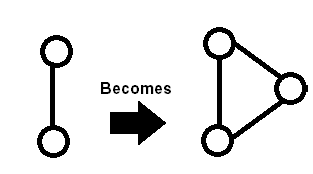
\includegraphics{red20.png}
	\label{fig:red20}
\end{figure}
Since Vertex Cover is concerned with the vertices including the edges and dominating set is interested specifically in the vertices,
adding these new vertices as representations of the edges ensures that the resulting dominating set is a vertex cover. Additionally,
none of these new additional vertices should be selected as one of the dominating set, due to how they are connected into the graph. 
If one is selected there will always be a smaller dominating set that does no include that outside connection. 

\newpage

23. In the disjoint paths problem the input is a directed graph $G$ and pairs $(s_1, t_1), \ldots, (s_k, t_k)$ of vertices.
The problem is to determine if there exist a collection of vertex disjoint paths between the pairs of
vertices (from each $s_i$ to each $t_i$). Show that this problem is NP-hard by a reduction from the 3SAT
problem. Note that this problem is not easy.\\
HINT: Construct one pair ($s_i, t_i)$ for each variable $x_i$ in your formula $F$ . Intuitively there will be
two possible paths between $s_i$ and $t_i$ depending on whether $x_i$ is true or false. There will be a
component/subgraph $D_j$ of $G$ for each clause $C_j$ in $F$. There will be three possible paths between the
$(s_i, t_i)$'s pairs for each $D_j$ . You want that it is possible to route any two of these paths (but not all
three) through $D_j$.
\newpage

2. You know that lots of famous computer scientists have tried to find a fast efficient parallel algorithm
for the following Boolean Formula Value Problem:\\
INPUT: A Boolean formula $F$ and a truth assignment $A$ of the variables in $F$.\\
OUTPUT: $1$ if $A$ makes $F$ true, and $0$ otherwise.\\
Moreover, most computer scientists believe that there is no fast efficient parallel algorithm for the
Boolean Value Problem. You want to find a fast efficient parallel algorithm for some new problem $N$.
After much effort you can not find a fast efficient parallel algorithm for $N$, nor a proof that $N$ does
not have a fast efficient parallel algorithm. How could you give evidence that finding a fast efficient
parallel algorithm for $N$ is at least a hard of a problem as finding a fast efficient parallel algorithm for
Boolean Formula Value problem? Be as specific as possible, and explain how convincing the evidence
is.\\
Note that ``fast and efficient'' means poly-log time with a polynomial number of processors. The term
``poly-log'' means bounded by O($log^kn$) for some constant $k$.\\
\\
With a standard reduction problem we create a polynomial time mapping from the input of Boolean Formula Value
problem to the input of $N$.\\
In parallel, we construct a parallel polynomial time mapping for the input of Boolean Formula Value to the
to the input of  $N$and demonstate that the Boolean Formula Value algorithm
returns a given result if and only if $N$ returns a certain result.\\
This shows that the Boolean Forumla Value algorithm will take at least the amount of time that $N$
takes. Since, we do not have a fast efficient parallel algorithm
for the Boolean Formula Value Problem we must not have one for $N$.
\newpage

3. Consider the problem of taking as input an integer $n$ and an integer $x$, and creating an array $A$ of $n$
integers, where each entry of $A$ is equal to $x$.\\

Give an algorithm runs in time O($log~n$) on a EREW PRAM using $n$ processors. What is the
efficiency of this algorithm?\\
\\
The algorithm works as follows:\\
Assign($1, \ldots, n/2$, $n/2$), Assign($n/2 + 1, \ldots, n$, $n/2$)\\ 
where Assign us a recursive call to assign $x$ to the $i$th location in the array.\\
The resulting call tree has a height of $log~n$, and $n$ leaves.\\
T($n$, $p$) calls two parallel calls requiring T($n/2$, $p/2$). From this we 
determine the efficiency to be: $n/n(1 + lg~n) =  1/(1+ lg~n)$, since the time spent in an 
individual leaf will be 1 time unit performing the assignment.\\ 
\\
Give an algorithm that runs in time O($log~n$) on a EREW PRAM using $n/log~n$ processors. What
is the efficiency of this algorithm?\\
\\
The recurrence relation is the same as the previous problem, but the value of $p$ has changed.\\
The height of this tree is $log~p$ = $log(n/log~n)$ and the time spent in an individual leaf is $log~n$.\\ 
Using the same algorithm as above we calculate the efficiency as:\\
	\[
	E(n,p) = \frac{log(n)}{log(n)+log(\frac{n}{log(n)})}
\]
\\
\\
Give an algorithm that runs in time O(1) on a CRCW PRAM using $n$ processors. What is the
efficiency of this algorithm?\\
In one time step, each processor reads $x$ and writes to a location in $A$. This algorithm requires
a CREW machine. T($n$,$p$) calls $n$ parallel calls requiring O(1) time, with a call tree of height one.
The efficiency is: $\frac{S(n)}{p~\mdot~T(n,p)} = \frac{n}{n~\mdot~1} = 1$.
\\

\end{document}
